\aufgabe{}{

You received a dataset with 11 observations and two features:

\begin{table}[ht]
\centering
\begin{tabular}{rrrrrrrrrrrr|r}
\hline
& 1 & 2 & 3 & 4 & 5 & 6 & 7 & 8 & 9 & 10 & 11 & $\sum_{i = 1}^n$ \\ 
\hline
y & -7.90 & -6.08 & -3.74 & -1.18 & -1.23 & -0.55 & 0.05 & 0.88 & 4.74 & 2.93 & 2.55 & -9.53\\ 
x1 & -1.00 & -0.80 & -0.60 & -0.40 & -0.20 & 0.00 & 0.20 & 0.40 & 0.60 & 0.80 & 1.00 & 0 \\ 
x2 & 0.95 & 0.65 & 0.40 & 0.07 & 0.06 & 0.02 & 0.02 & 0.14 & 0.34 & 0.60 & 0.98 & 4.23 \\ 
\hline
\end{tabular}
\end{table}

The last column corresponds to the sum of values of each row.

\begin{enumerate}[a)]
\item Compute the Pearson correlation of $x_1$ and $x_2$.  
The formula is: 
$$ 
\rho(x_1, x_2) = \frac{\sum_{i = 1}^n (x_1^{(i)} - \overline{x}_1)(x_2^{(i)} - \overline{x}_2)}{\sqrt{\sum_{i = 1}^n (x_1^{(i)} - \overline{x}_1)^2} \sqrt{\sum_{i = 1}^n (x_2^{(i)} - \overline{x}_2)^2}}
$$ 
To speed up things, the individual differences to the means ($x_1^{(i)} - \overline{x_1}$, $x_2^{(i)} - \overline{x_2}$),  are given in the table above.  

\begin{table}[h]
\centering
\begin{tabular}{rrrrrrrrrrrr}
\hline
& 1 & 2 & 3 & 4 & 5 & 6 & 7 & 8 & 9 & 10 & 11 \\ 
\hline
$x_1^{(i)} - \overline{x_1}$ & -1.00 & -0.80 & -0.60 & -0.40 & -0.20 & 0.00 & 0.20 & 0.40 & 0.60 & 0.80 & 1.00 \\ 
$x_2^{(i)} - \overline{x_2}$ & 0.57 & 0.27 & 0.02 & -0.31 & -0.32 & -0.36 & -0.36 & -0.24 & -0.04 & 0.22 & 0.6 \\ 
\hline
\end{tabular}
\end{table}

Interprete the results. Based on $\rho(x_1, x_2)$, are $x_1$ and $x_2$ correlated? 

\item Add points ($x_1$, $x_2$) to the following figure: 


\begin{figure}[!ht]
\centering
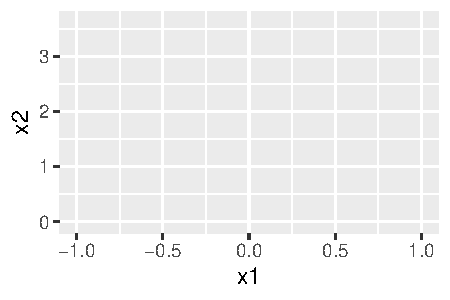
\includegraphics[width=\maxwidth]{figure/add_Points_x1_x2.pdf}]

\end{figure}


Based on your drawing, do you consider the Pearson correlation coefficient a reliable measure to 
detect dependencies for the above use case?

\item One method to detect non-linear relationships is the usage of 
generalized additive models (GAM).
The following shows the output of the GAM when $x_2$ depends on a smooth function of $x_1$. 

\verbatiminput{rsrc/GAM_Output.txt} 

What conclusions could you draw for the relationship between $x_1$ and $x_2$? 

\item 
Instead of 11 datapoints you received a dataset with 1000 datapoints from 
the same data generating process as above. 
You fitted a linear model to the data 
$\fh(\xv) = \hat \beta_0 + \hat\beta_1 \xv_1 + \hat\beta_2 \xv_2 + \hat\beta_3 \xv_1 \xv_2$
The following plots show the PDP (first row) and ALE (second row) for $x_1$ and $x_2$. 
\begin{enumerate}
\item Interprete the plots with respect to the feature effect of $x_1$ and $x_2$. 
\item Would you rather trust the PDP or ALE plot? Give reasons for your 
decision. 



\begin{center}
  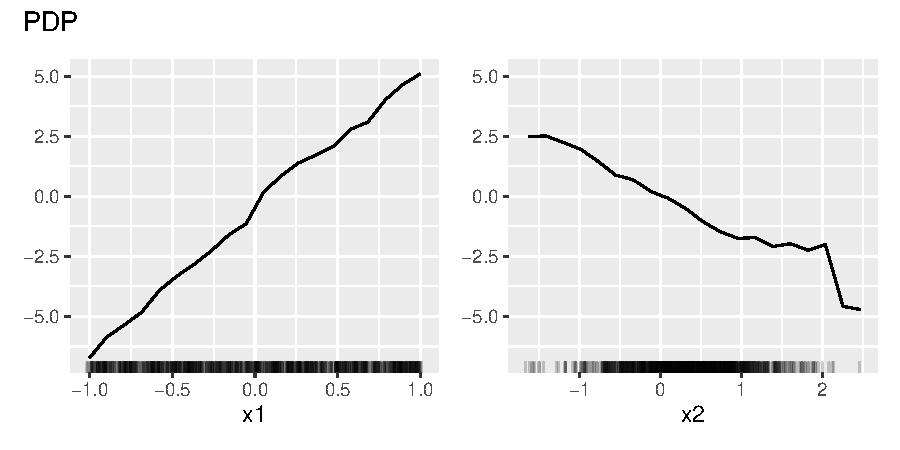
\includegraphics[width=\maxwidth]{figure/PDP_Plot.pdf}
\end{center}


\begin{center}
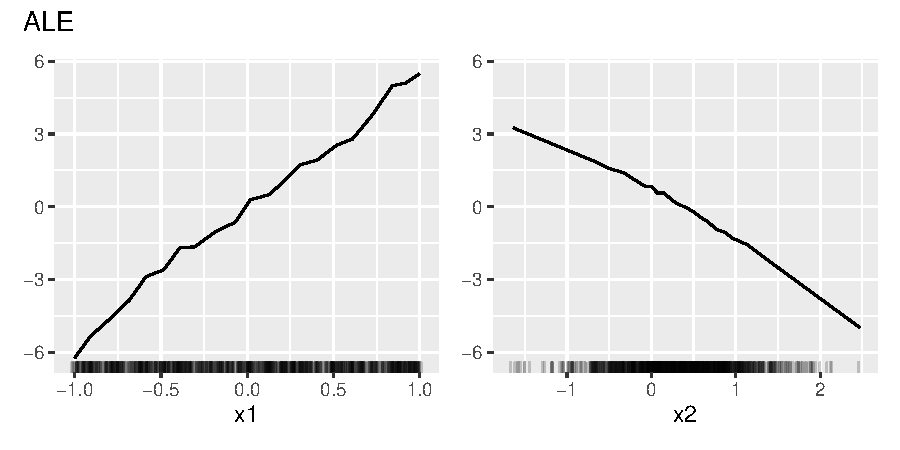
\includegraphics[width=\maxwidth]{figure/ALE_Plot.pdf}
\end{center}



\end{enumerate}
\end{enumerate}
}
